%!TEX root = ../master.tex
\chapter{Implementation}\label{ch:implementation}

\section{Tools used}\label{sec:toolsused}
!Anna rettelse. Tjek om ok eller ej!
The tools used in this project is an Arduino and the software Pure Data. 
An Arduino is a micro controller that allows the user to code and create their own circuits using various components. The Arudino is responsible for the control of the physical interface which the user has available.
Pure data is a C/C++ based coding language which utilises pre-constructed blocks of code which have to be connected to one another. Pure data is the code implemented in the project which is responsible for the audio and image processing. The image processing is conducted by utilising a library called Gem. 
A library called Firmata allows the Arduino to communicate with the software on the laptop.


!Before!
The tools used in this project is Pure data and Arduino. 
Pure data is a C/C++ based coding language which utilises pre-constructed blocks of code which have to be connected to one another. Pure data is the code implemented in our project which is responsible for the audio and image processing. Gem is used for the image processing purpose, which is a library in Pura data that allows for various image processing and animation methods.  
Furthermore three different filters have been constructed and implemented using pure data.

An Arduino is a micro controller that allows the user to code and create their own circuits using various components, this allows for a wide range of purposes. In this project the Arudino is responsible for the physical interface which the user has available. 

\subsection{Audio filters}
In the domain of audio effects, the term "filters" describes effects that modify the partial amplitudes of audio signals according to their frequencies \cite{zolzer2011dafx}. Filters combine their input signal with delayed and modified versions of themselves and then filters out certain frequencies. If a delayed version of the input signal is added to the signal, it is called a feedfoward filter, and if the signal is added to a delayed version of itself, it is called a feedback filter. This makes feedback filters more tricky to work with, since their effects can essentially amplify themselves \cite{steiglitz1997digital}. In this case the amplification can continue forever, no matter if you feed the filter a new input signal or not. This continuous amplification is called an unstable filter. Inversely, a stable filter is one, where the response fades over time, tending towards zero. This way, you make sure that the response of the input signal will end, depending on how fast the response signal fades.

\begin{figure}
\centering
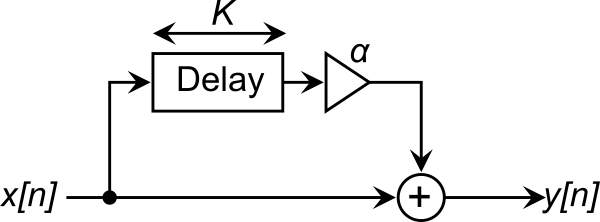
\includegraphics[width=0.5\textwidth]{feedforward}
\caption{Structure of basic feedforward filter.}
\label{fig:feedforward}
\end{figure}

\begin{figure}
\centering
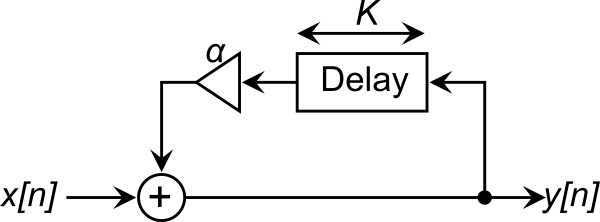
\includegraphics[width=0.5\textwidth]{feedback}
\caption{Structure of basic feedback filter.}
\label{fig:feedback}
\end{figure}

Filters can be put into three basic categories:
\begin{itemize}
\item \textbf{Pass filters} which lets defined frequencies pass, and reject the remaining. Examples of this type of filter are low-pass, bandpass and comb filters.
\item \textbf{Reject Filters} which is the inverse of a Pass filter. With this, defined frequencies are rejected and lets the remaining frequencies pass. Bandreject filters, also known as notch filters, are an example of this.
\item \textbf{Equaliser filters} which changes the amplitude of defined frequencies. This amplitude change can either be positive or negative, depending on the specific implementation of the filter. 
\end{itemize}

The filters used in the project is a bandpass, comb and high-shelf.

The comb filter used is a simple feedback filter, of the structure seen in Figure \ref{fig:feedback}. The summation of the delays creates constructive and destructive interference on the signal. This interference is at regular intervals, which gives the curve of the frequency response its distinct appearance, as seen in Figure \ref{fig:comb}. It is used to give an echo-like effect unto the input signal.

\begin{figure}
\centering
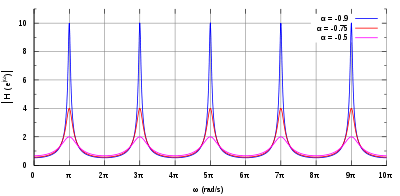
\includegraphics[width=0.5\textwidth]{comb}
\caption{Frequency response curve of comb filter.}
\label{fig:comb}
\end{figure}

The two other filters used are structured as biquads. \todo{CONTINUE FROM HERE}

The bandpass filter works by letting certain frequencies pass through, while rejecting all other frequencies. The accepted frequencies are defined by having a band with width \(B\) and a frequency \(f_0\) as its  centre point. This structure can be seen in Figure \ref{fig:bandpass}. The outermost points of the band \(f_L\) and \(f_H\) define the lowest and highest frequencies that are passed through, respectively. All frequencies lower than \(f_L\) and higher than \(f_H\) are rejected.

\begin{figure}
\centering
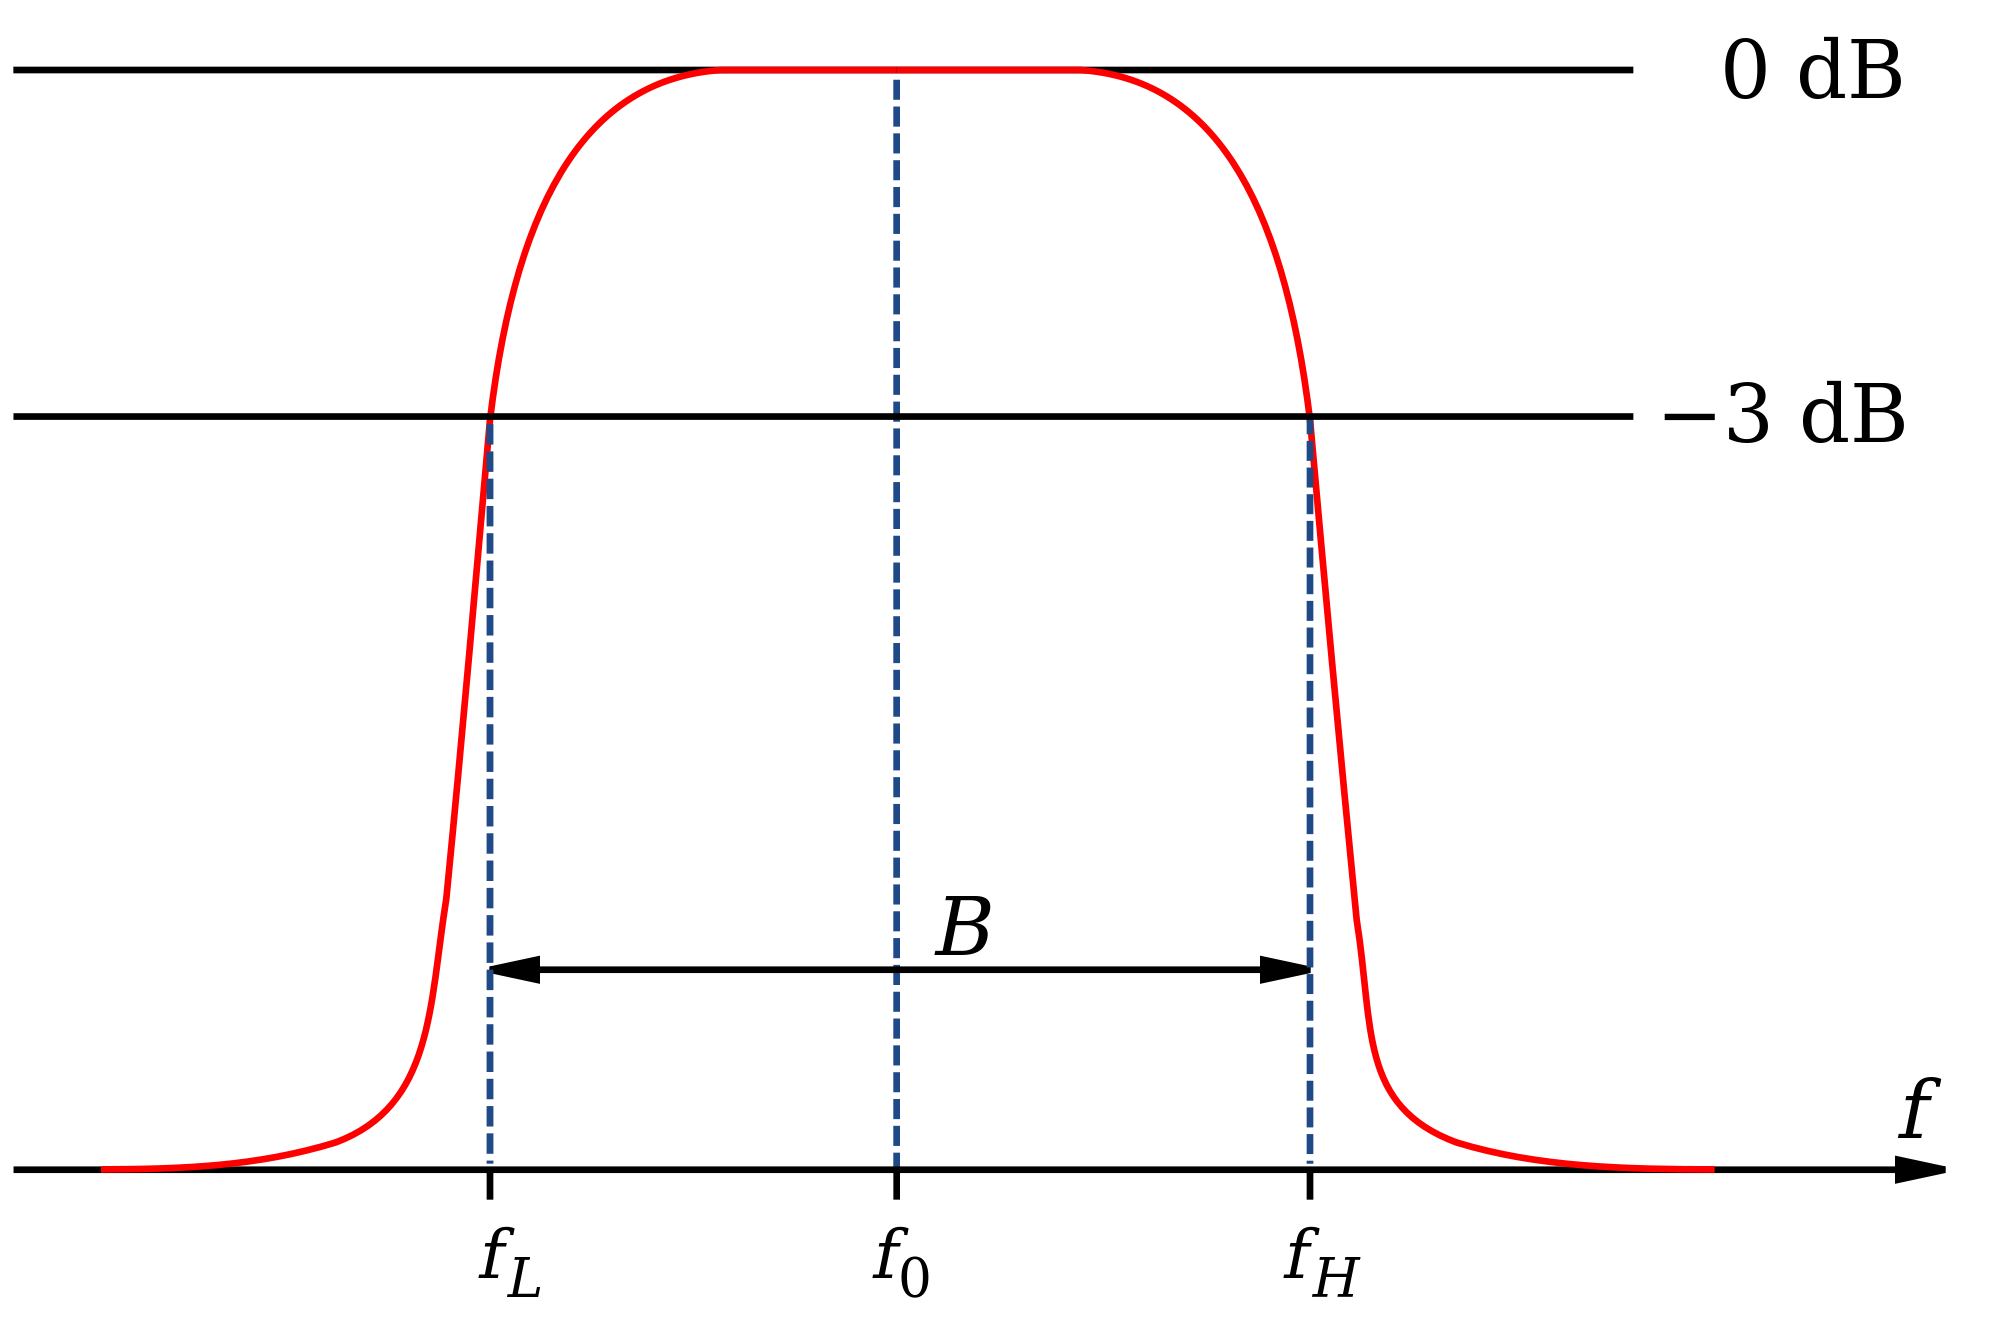
\includegraphics[width=0.5\textwidth]{bandpass}
\caption{Frequency response curve of bandpass filter.}
\label{fig:bandpass}
\end{figure}

\section{Software tools}\label{sec:softwareTools}
	\subsection{Image processing}\label{sub:imageprocessing}
	As the project revolves around pictures being audiolised, various image processing methods have been implemented. To get an image loaded into Pure data the library gem have been imported and applied. In gem it is possible to go through each pixel getting its RGB value as three different values. This is done using a double nested for-loop that is constructed using the expr function in Pure data, which allows for construction of consecutive if-statements. The first if-statement gives an output that is increased by 0.001 for every cycle if the input value is less than one. The second if-statement checks if the input value is greater or equal to one, if that is the case it adds 0.01 to a value starting at zero, which is then outputted. The last if-statement checks if the second input is greater or equal to 1, if that is the case subtract 1 from the value of the second input.
	
	Pipe is an object that delay the input given to it by a specific amount of milliseconds. It is used here to make sure that the program does not give a stack overflow error, and that it doesn't process the pixels too fast. By default in the program the pipe is set to 50 milliseconds since this allows the program to smoothly go through each pixel one by one. 
	When the pixel data is being processed in the program, it outputs the value of the three colour channels in the specific pixel, meaning that the output consists of three different value representing the R, G and B value. With the three RGB values it is possible to plot the values giving a graph of how the colour distribution is in the picture, but it is also possible to normalize the values into a signal by normalizing them from zero to one into negative one to positive one. By doing this the values have now been turned into a signal, which in terms should be able to produce a sound.

	\subsection{Audiolisation of image}\label{sub:audiolisationofimage} 
	Audiolisation of an image means to turn the image into some kind of audio, which is what the program explained in \ref{sub:imageprocessing} is programmed to do. 
	
	\subsection{Arduino}\label{sub:arduino}
	Arduino is a micro controller with open source software, that allows for custom coding in processing. Arduino has the capability to be connected to a breadboard for greater utility as the breadboard allows multiple components to be connected to a single Ardunio port, making it possible to create a 5 volt circuit using only a single pin. It is also possible to create a circuit using more than one pin, giving access to greater utility as each pin can be programmed separately in the program, giving each of the pins a unique functionality or making them become a duplicate, this would allow each pin to run a different circuit.
	Arduino is used in the project as the main control unit, as it is connects the physical interface to pure data. 
	
\section{Physical interface}\label{sec:physicalinterface}

	
	\subsection{Circuit diagram}\label{sub:circuitdiagram}
\begin{figure}
\centering
\includegraphics[width=0.5\textwidth]{circuit}
\caption{The circuit diagram.}
\label{fig:circuit}
\end{figure}

\begin{figure}
\centering
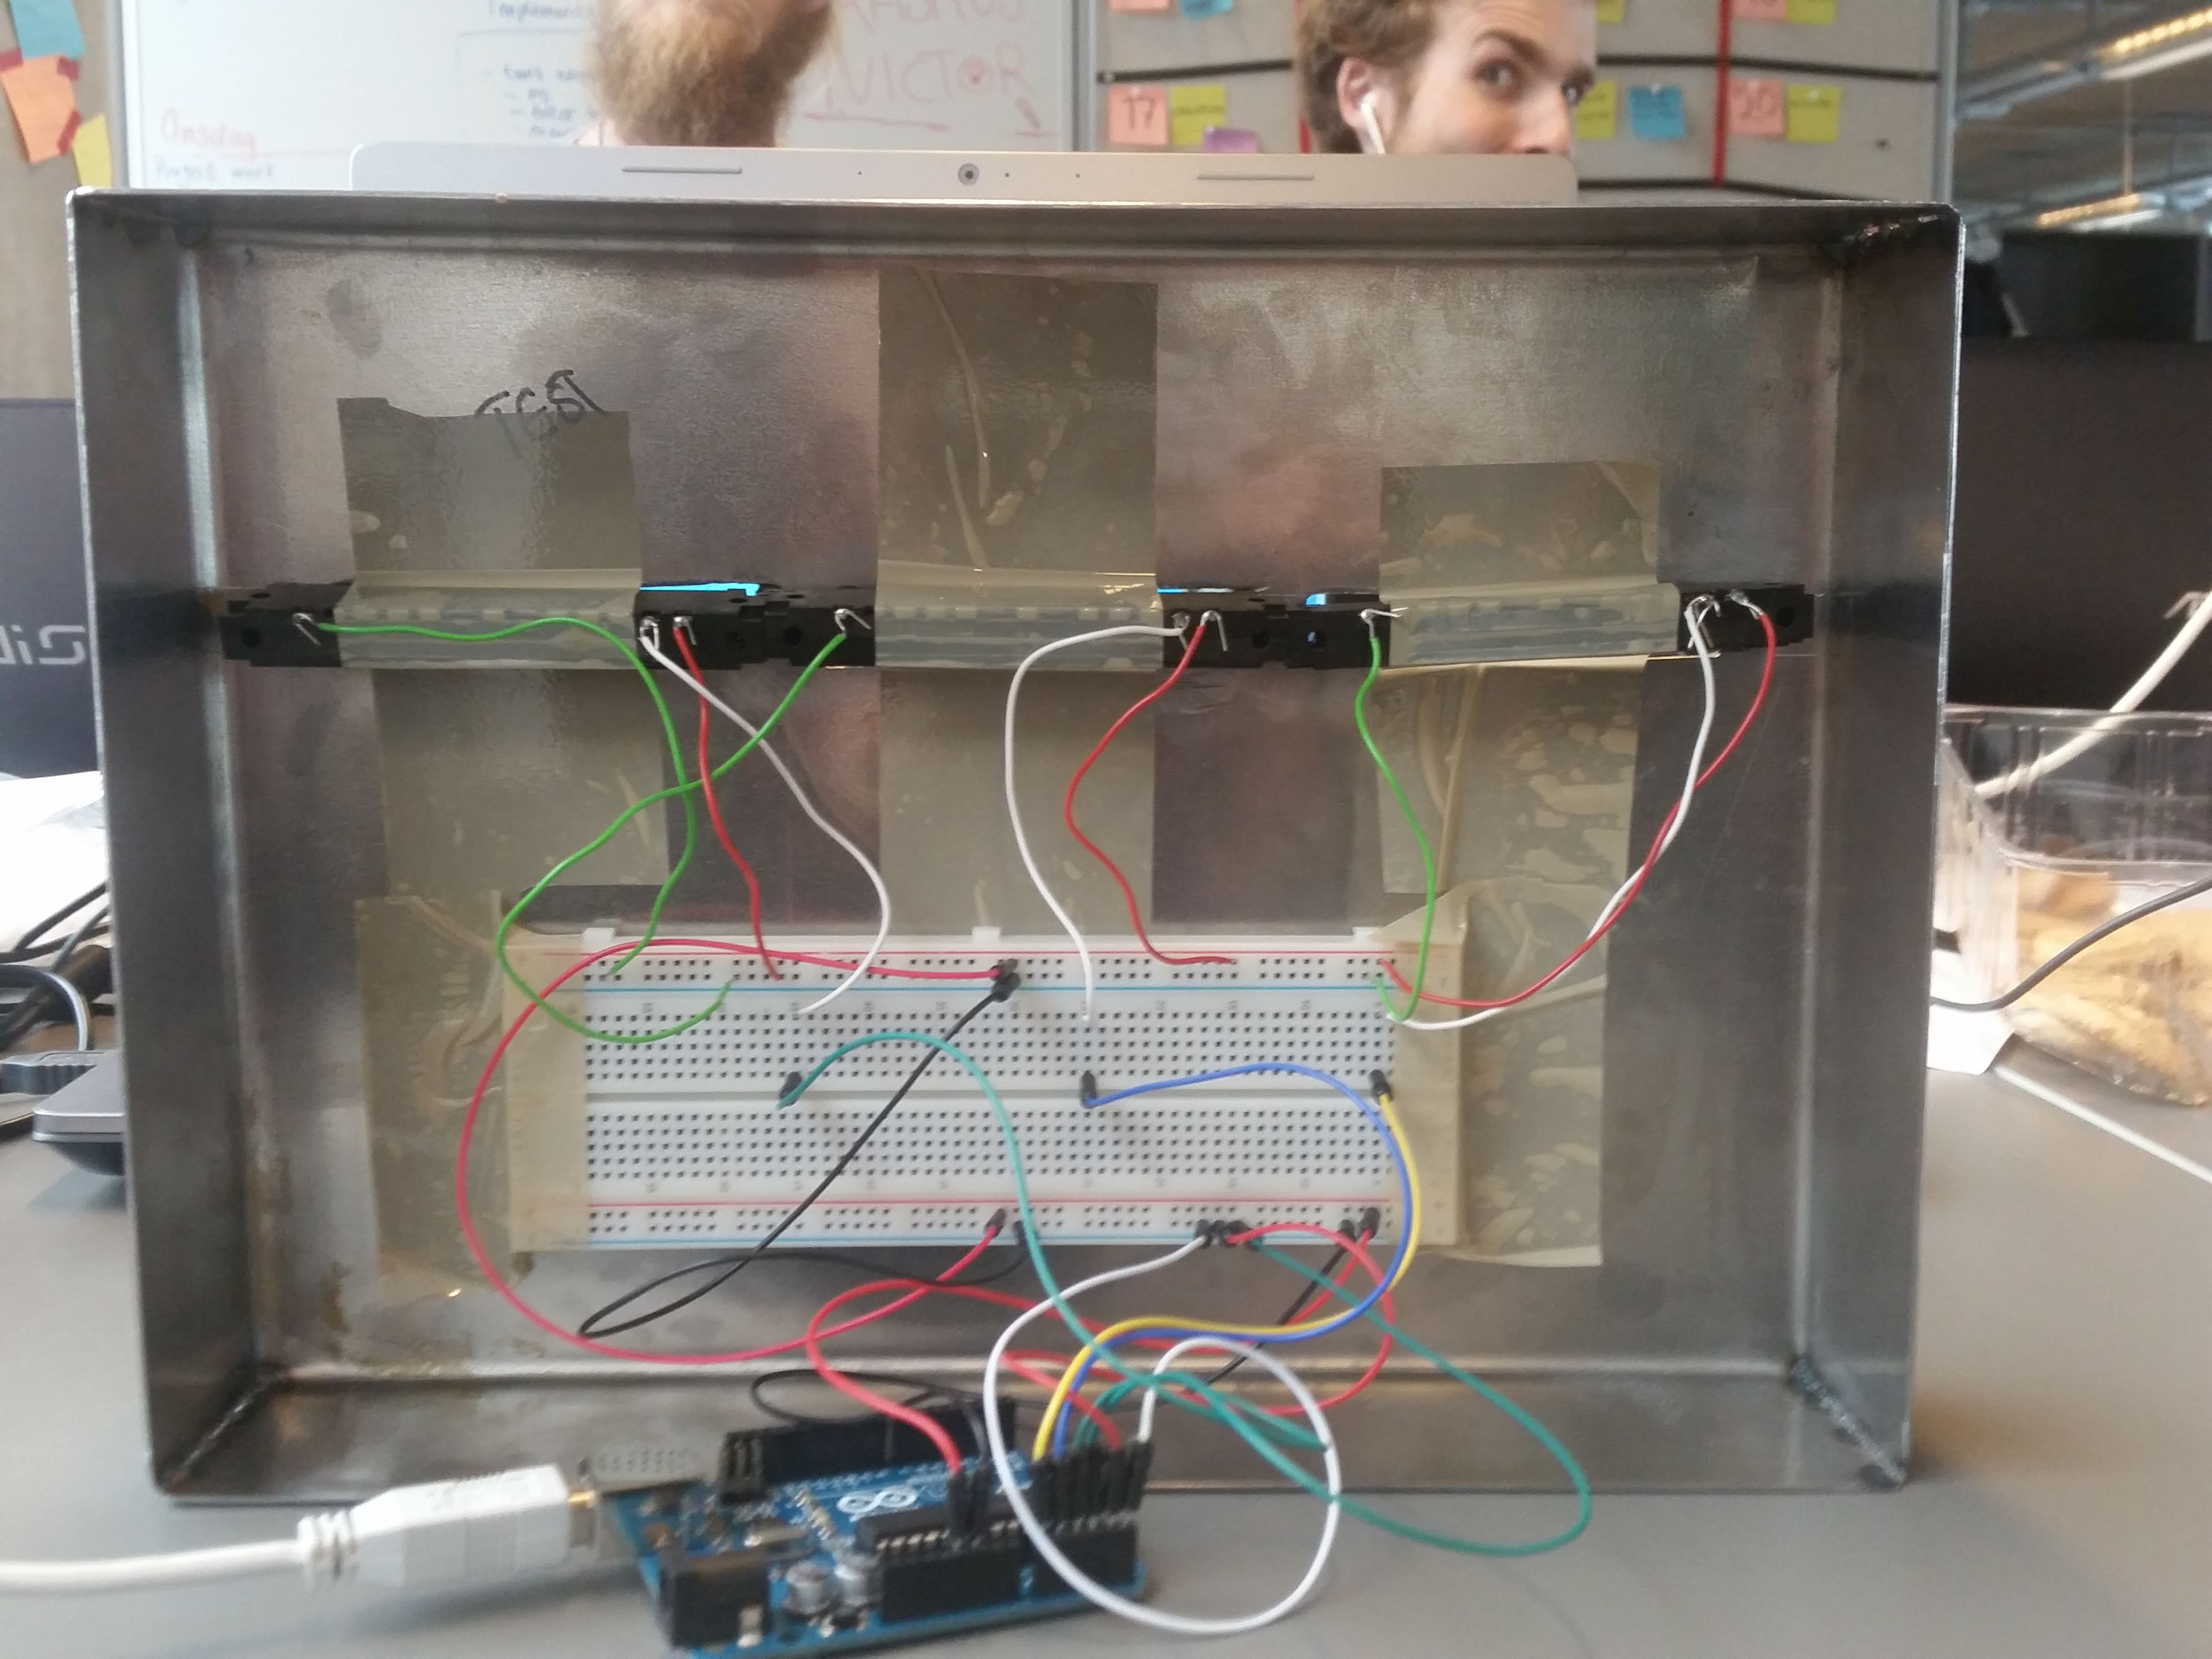
\includegraphics[width=0.5\textwidth]{backsideBox}
\caption{The circuit inside the box.}
\label{fig:backsideBox}
\end{figure}

\begin{figure}
\centering
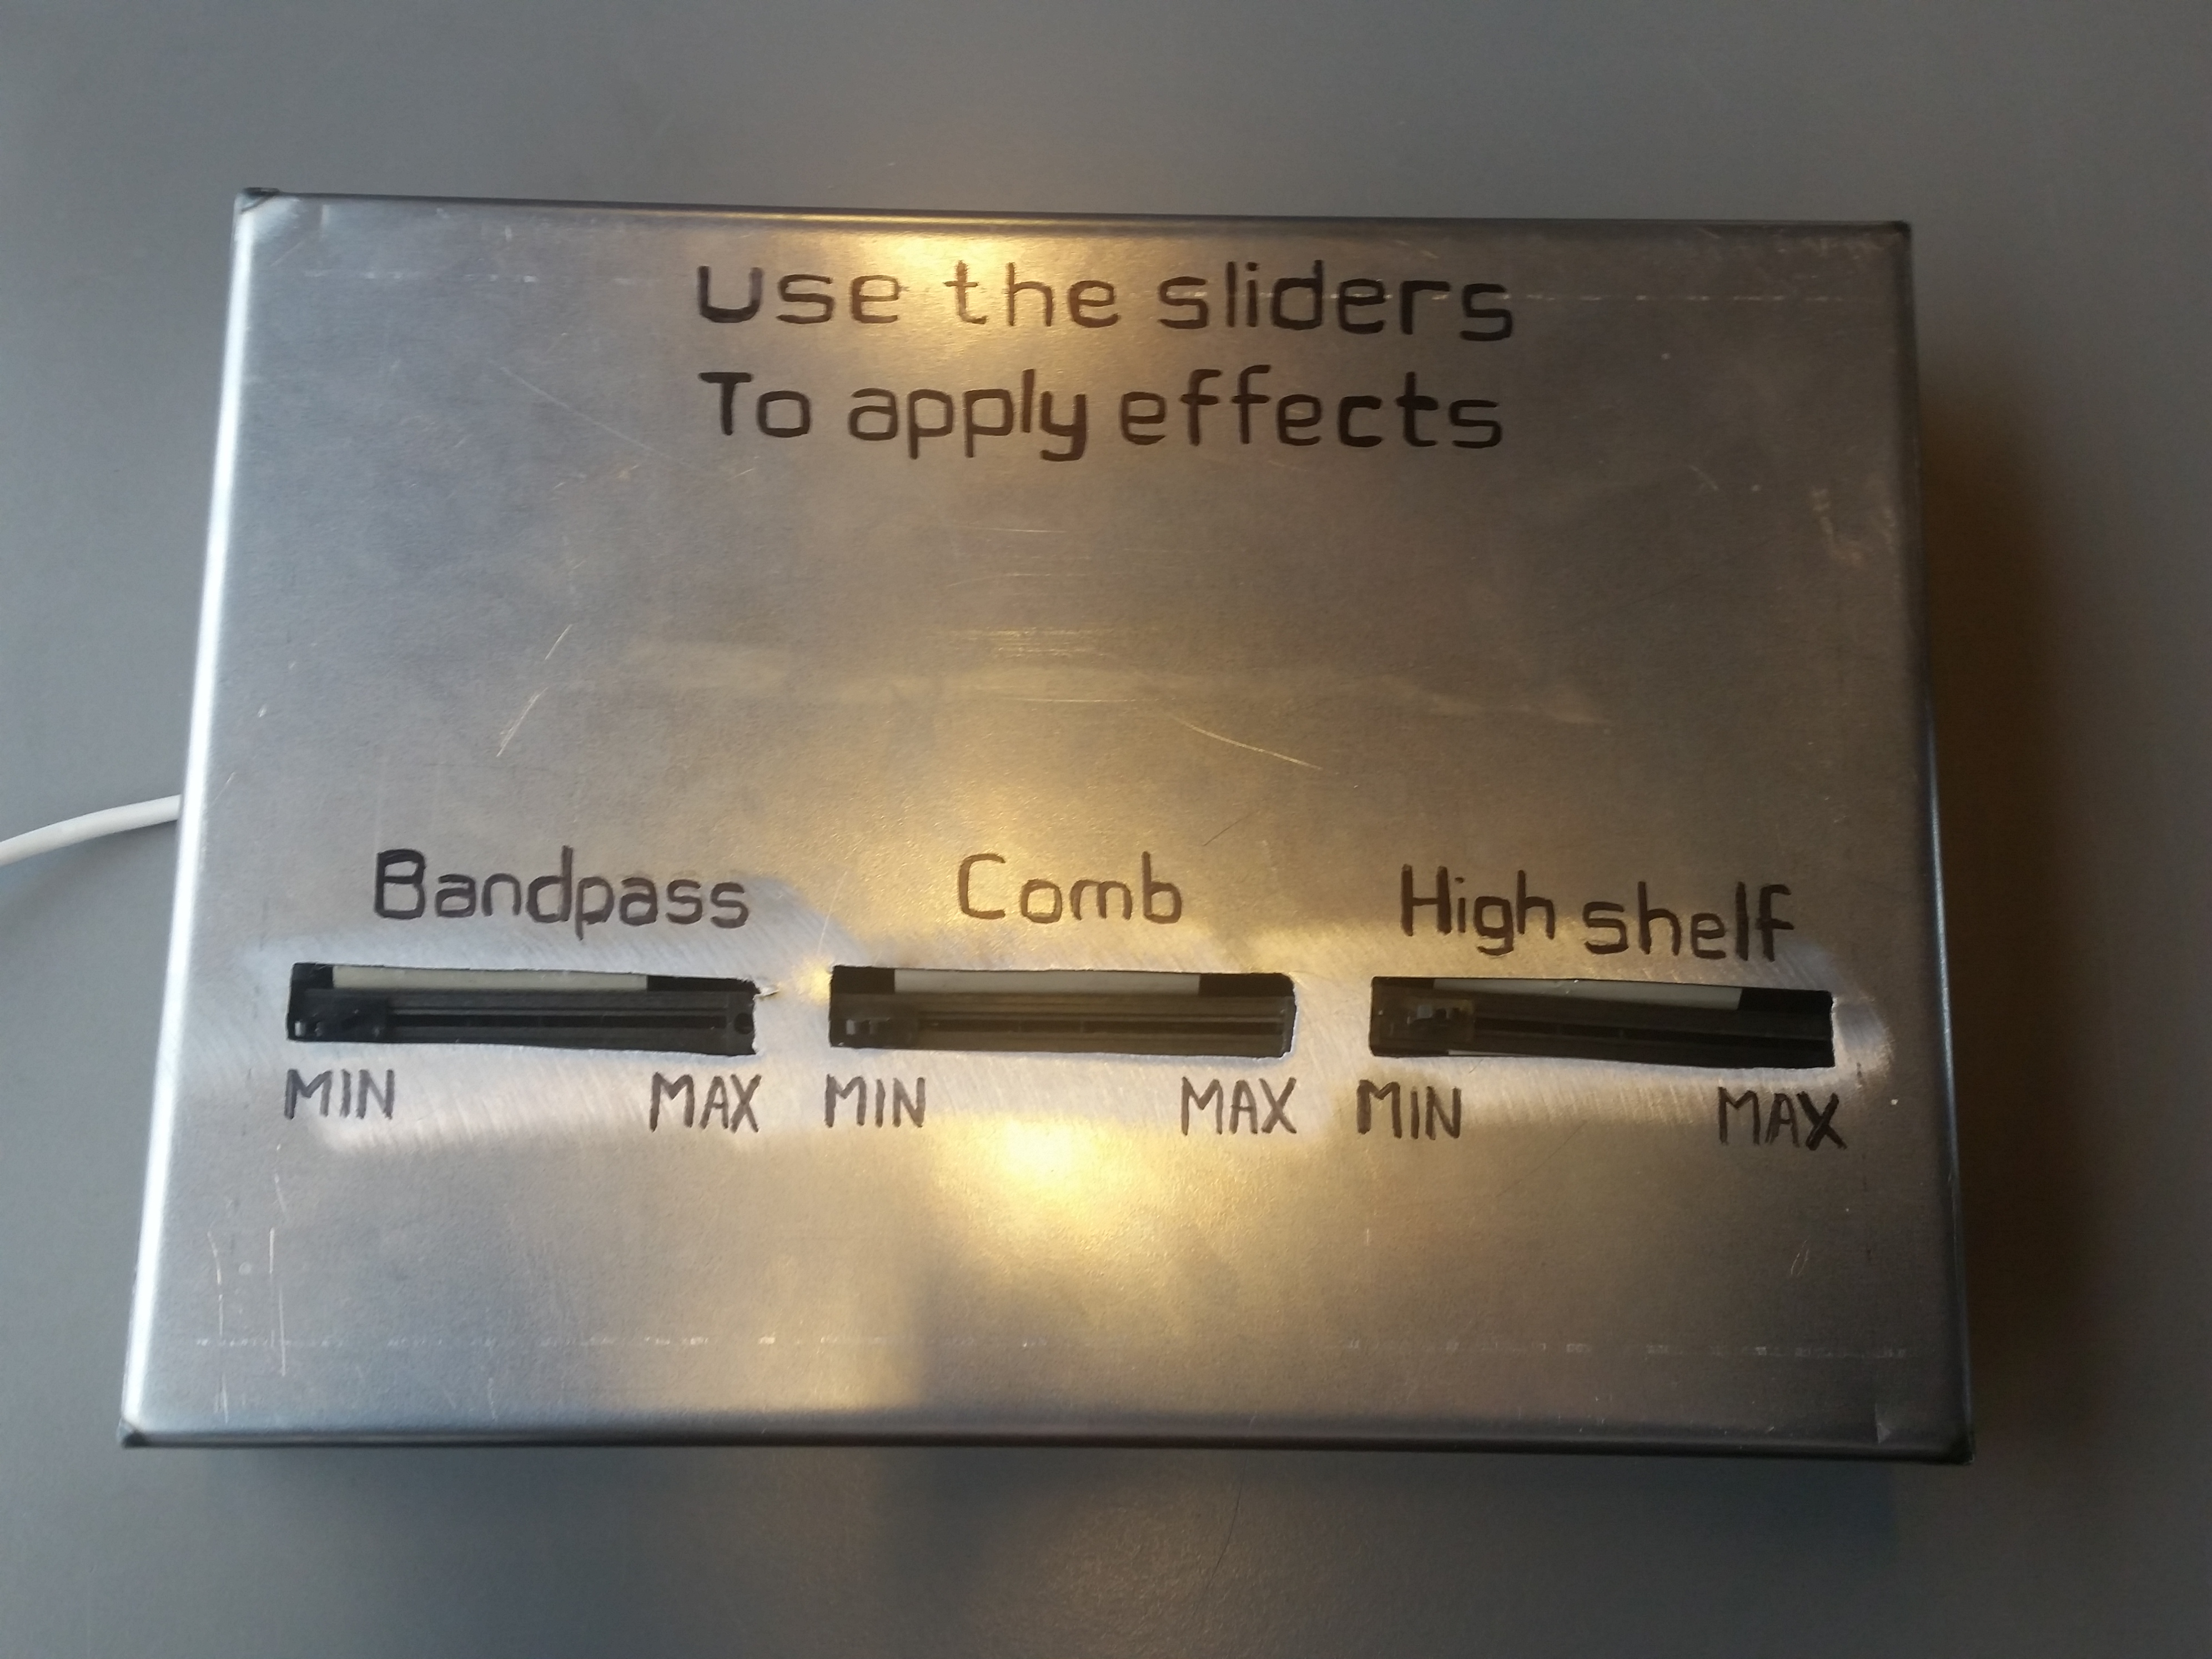
\includegraphics[width=0.5\textwidth]{frontBox}
\caption{The box containing the electronics.}
\label{fig:frontBox}
\end{figure}

	
	The interface works by utilising an Arduinos 5 Volt power supply and 3 slide potentiometer, placed in the lower half of the box, which send their output into the Arduino analogue ports, which is then interpreted by the code, which will be elaborated upon in Chapter \ref{ch:codeoverview} 
